\documentclass{article}
\usepackage[utf8]{inputenc}
\usepackage{graphicx}
\usepackage{lscape}
%\usepackage{hyperref}


\begin{document}

\listoffigures

\begin{figure}[htp]
    \centering
    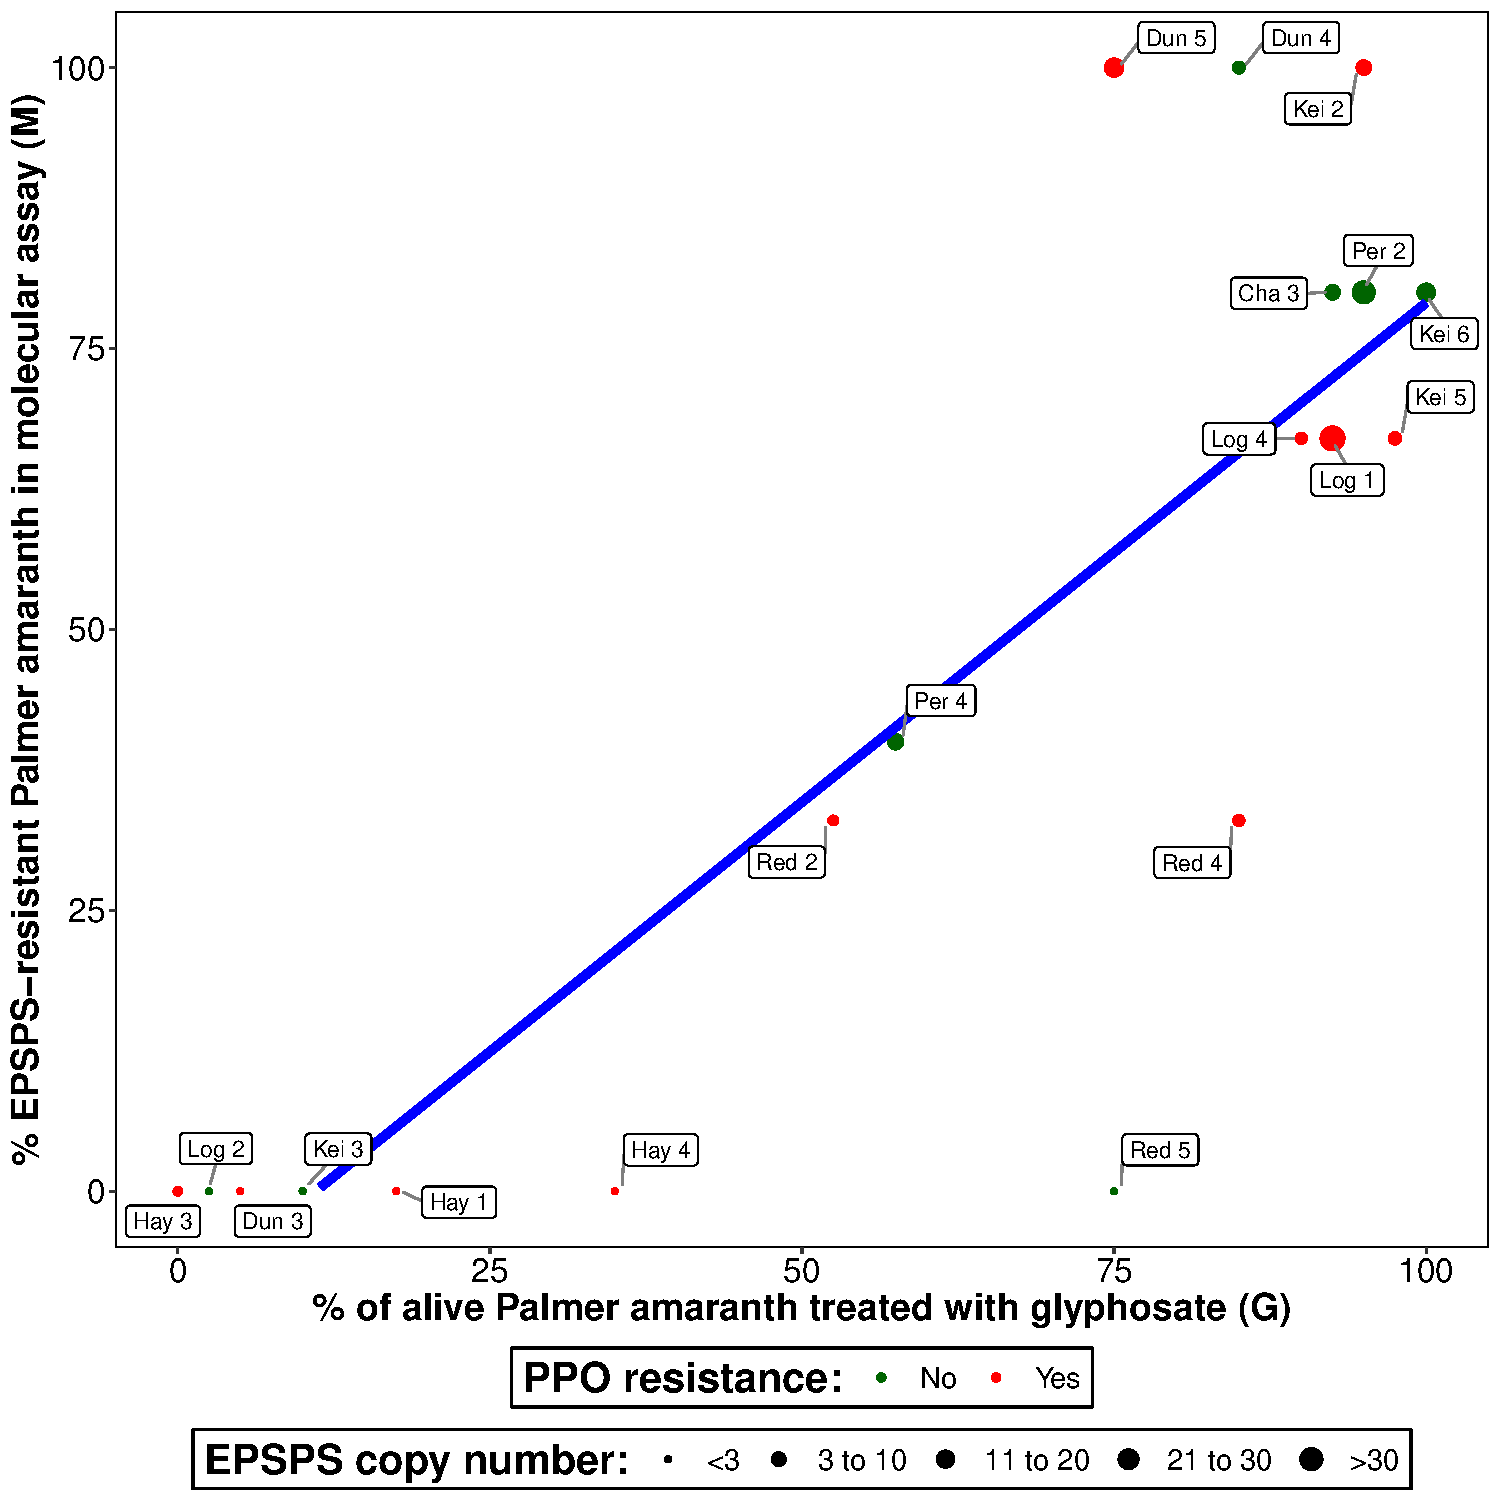
\includegraphics[width=14cm]{Figure 1.pdf}
    \caption{Correlation between EPSPS-inhibitor resistant \textit{Amaranthus palmeri} individuals with phenotypic (glyphosate) and genotypic (\textit{EPSPS} gene amplification) resistance assays. Dots are color coded to indicate resistance to PPO inhibitors, based on genotypic assays ($\triangle$G210 mutation).}
    \label{fig:galaxy}
\end{figure}



\begin{landscape}
\begin{figure}[htp]
    \centering
    \includegraphics[height=10cm]{Figure 2.pdf}
    \caption{Correlation between PPO-inhibitor resistant \textit{Amaranthus palmeri} individuals with phenotypic (fomesafen [A] and lactofen [B]) and genotypic ($\triangle$G210 mutation) resistance assays.}
    \label{fig:galaxy}
\end{figure}
\end{landscape}
 
 
 
\begin{landscape}
\begin{figure}[htp]
    \centering
    \includegraphics[height=10cm]{Figure 3.pdf}
    \caption{Presence of EPSPS- and/or PPO-inhibitor resistance based on genotypic resistance assay in 51 \textit{Amaranthus palmeri} populations from southwestern Nebraska.}
    \label{fig:galaxy}
\end{figure}
\end{landscape}
 
 

\begin{figure}[htp]
    \centering
    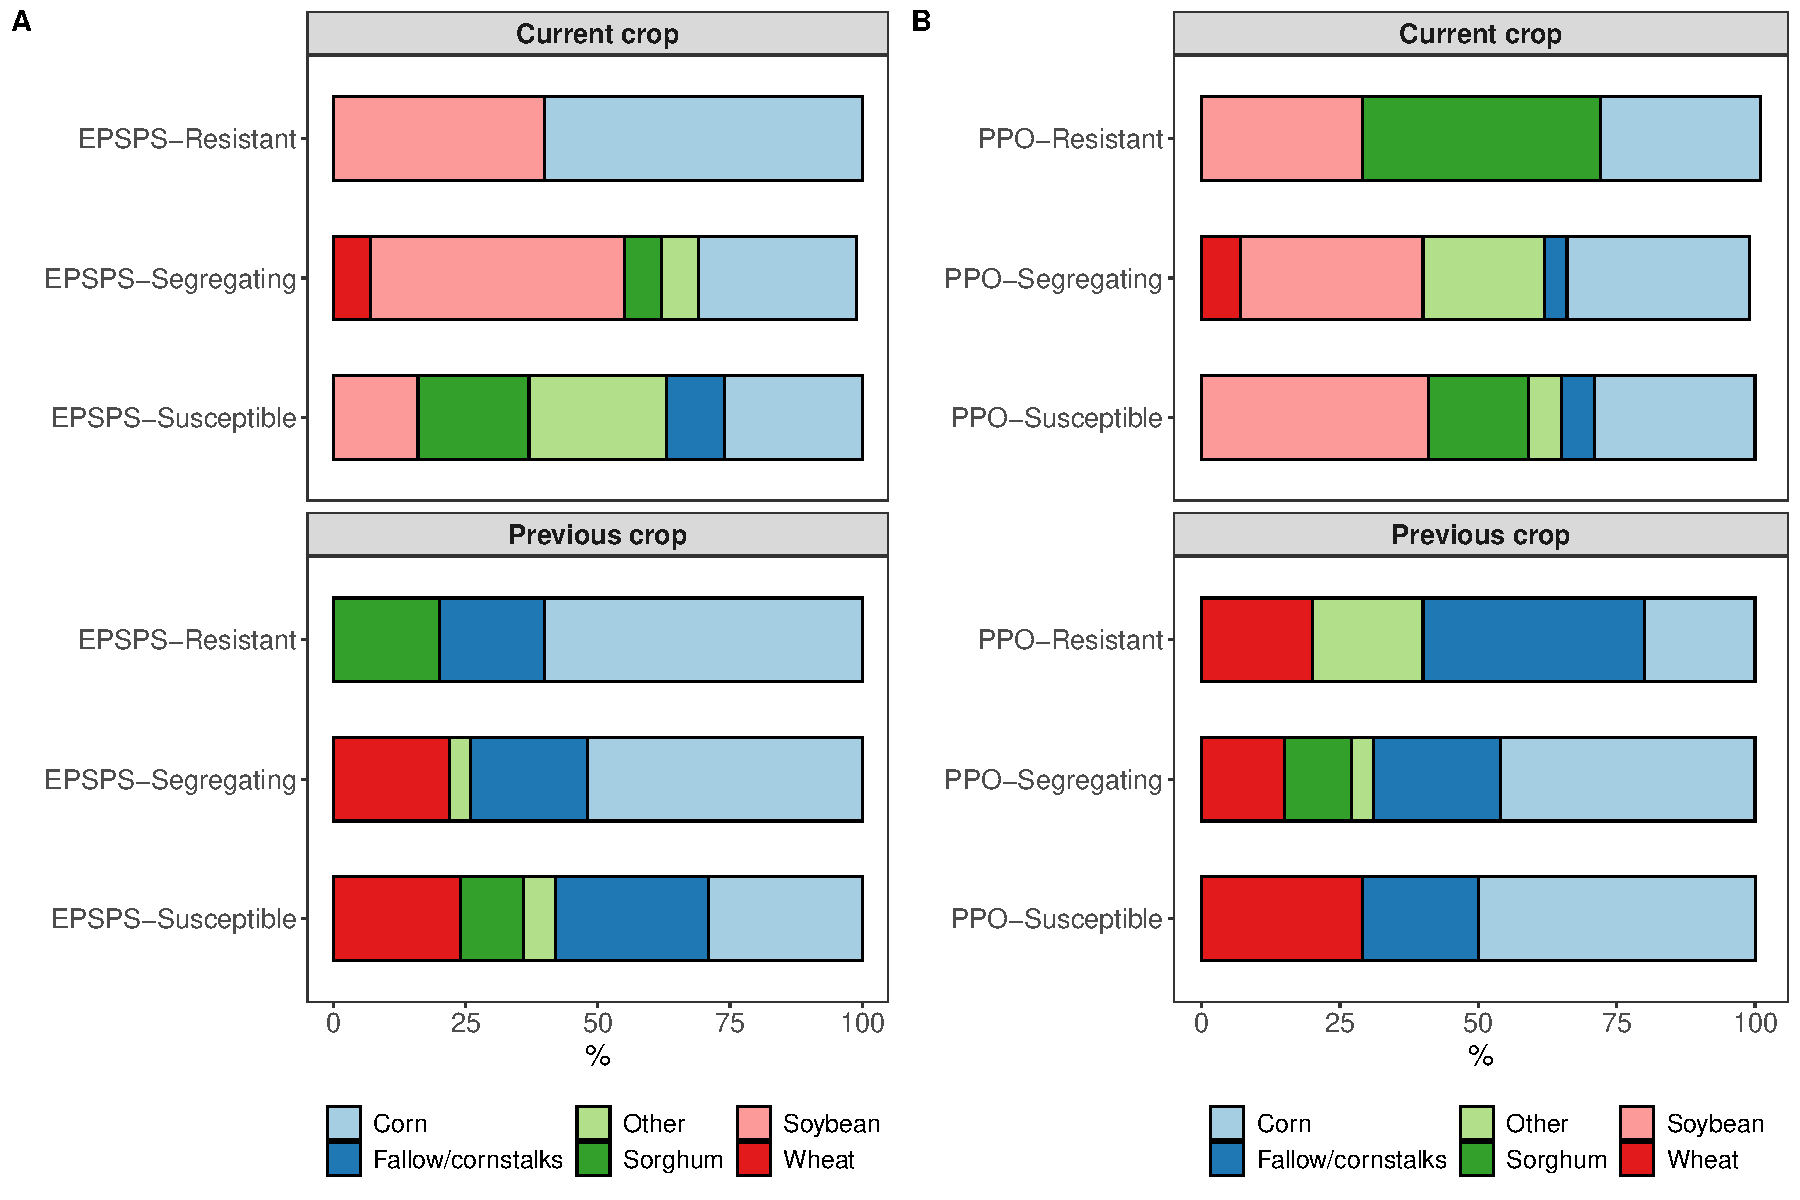
\includegraphics[height=11cm]{Figure 4.pdf}
    \caption{Random forest analysis of likelihood of EPSPS-inhibitor resistance (genotypic assay) in \textit{Amaranthus palmeri} populations in response to mechanism of resistance, agronomic practices, and geographic location and weed demographics in southwestern Nebraska. Variables are ordered by importance measured using the Gini coefficient.}
    \label{fig:galaxy}
\end{figure}



\begin{landscape}
\begin{figure}[htp]
    \centering
    \includegraphics[height=12cm]{Figure 5.pdf}
    \caption{Percentage of diversty in current and previous crop where the EPSPS-(A) and PPO-(B) resistant \textit{Amaranthus palmeri} populations was found in southwestern Nebraska. Based on genotypic resistance assay, populations are grouped into EPSPS- or PPO-Resistant, EPSPS- or PPO-Segregating and EPSPS- or PPO-Susceptible representing \textit{A. palmeri} with all resistant, partially resistant, and no resistant individuals, respectively. Other crops are represented by snap beans}
    \label{fig:galaxy}
\end{figure}
\end{landscape}


 
\end{document}
